\documentclass{jarticle}
\usepackage[dvipdfmx]{graphicx}
\usepackage{here}
\usepackage{listings}

\begin{document}

\title{最終課題}
\author{1029289895 尾崎翔太}
\date{2018/12/27}

\maketitle
\newpage

\section{システム概要}
レンタルビデオ屋のシステムを作った. 役割は課題1と同じだが, 機能は課題1とは大きく変わっている. 機能としてはユーザによる店舗検索と作品検索と履歴閲覧, 店員によるユーザ登録と貸出/返却, 管理者による店員の登録とメディアの登録と店の登録/削除及び店員がどの店で働くか, メディアをどの店に置くかの管理がある.

\section{実体関連図}
\begin{figure}[tp]
\begin{center}
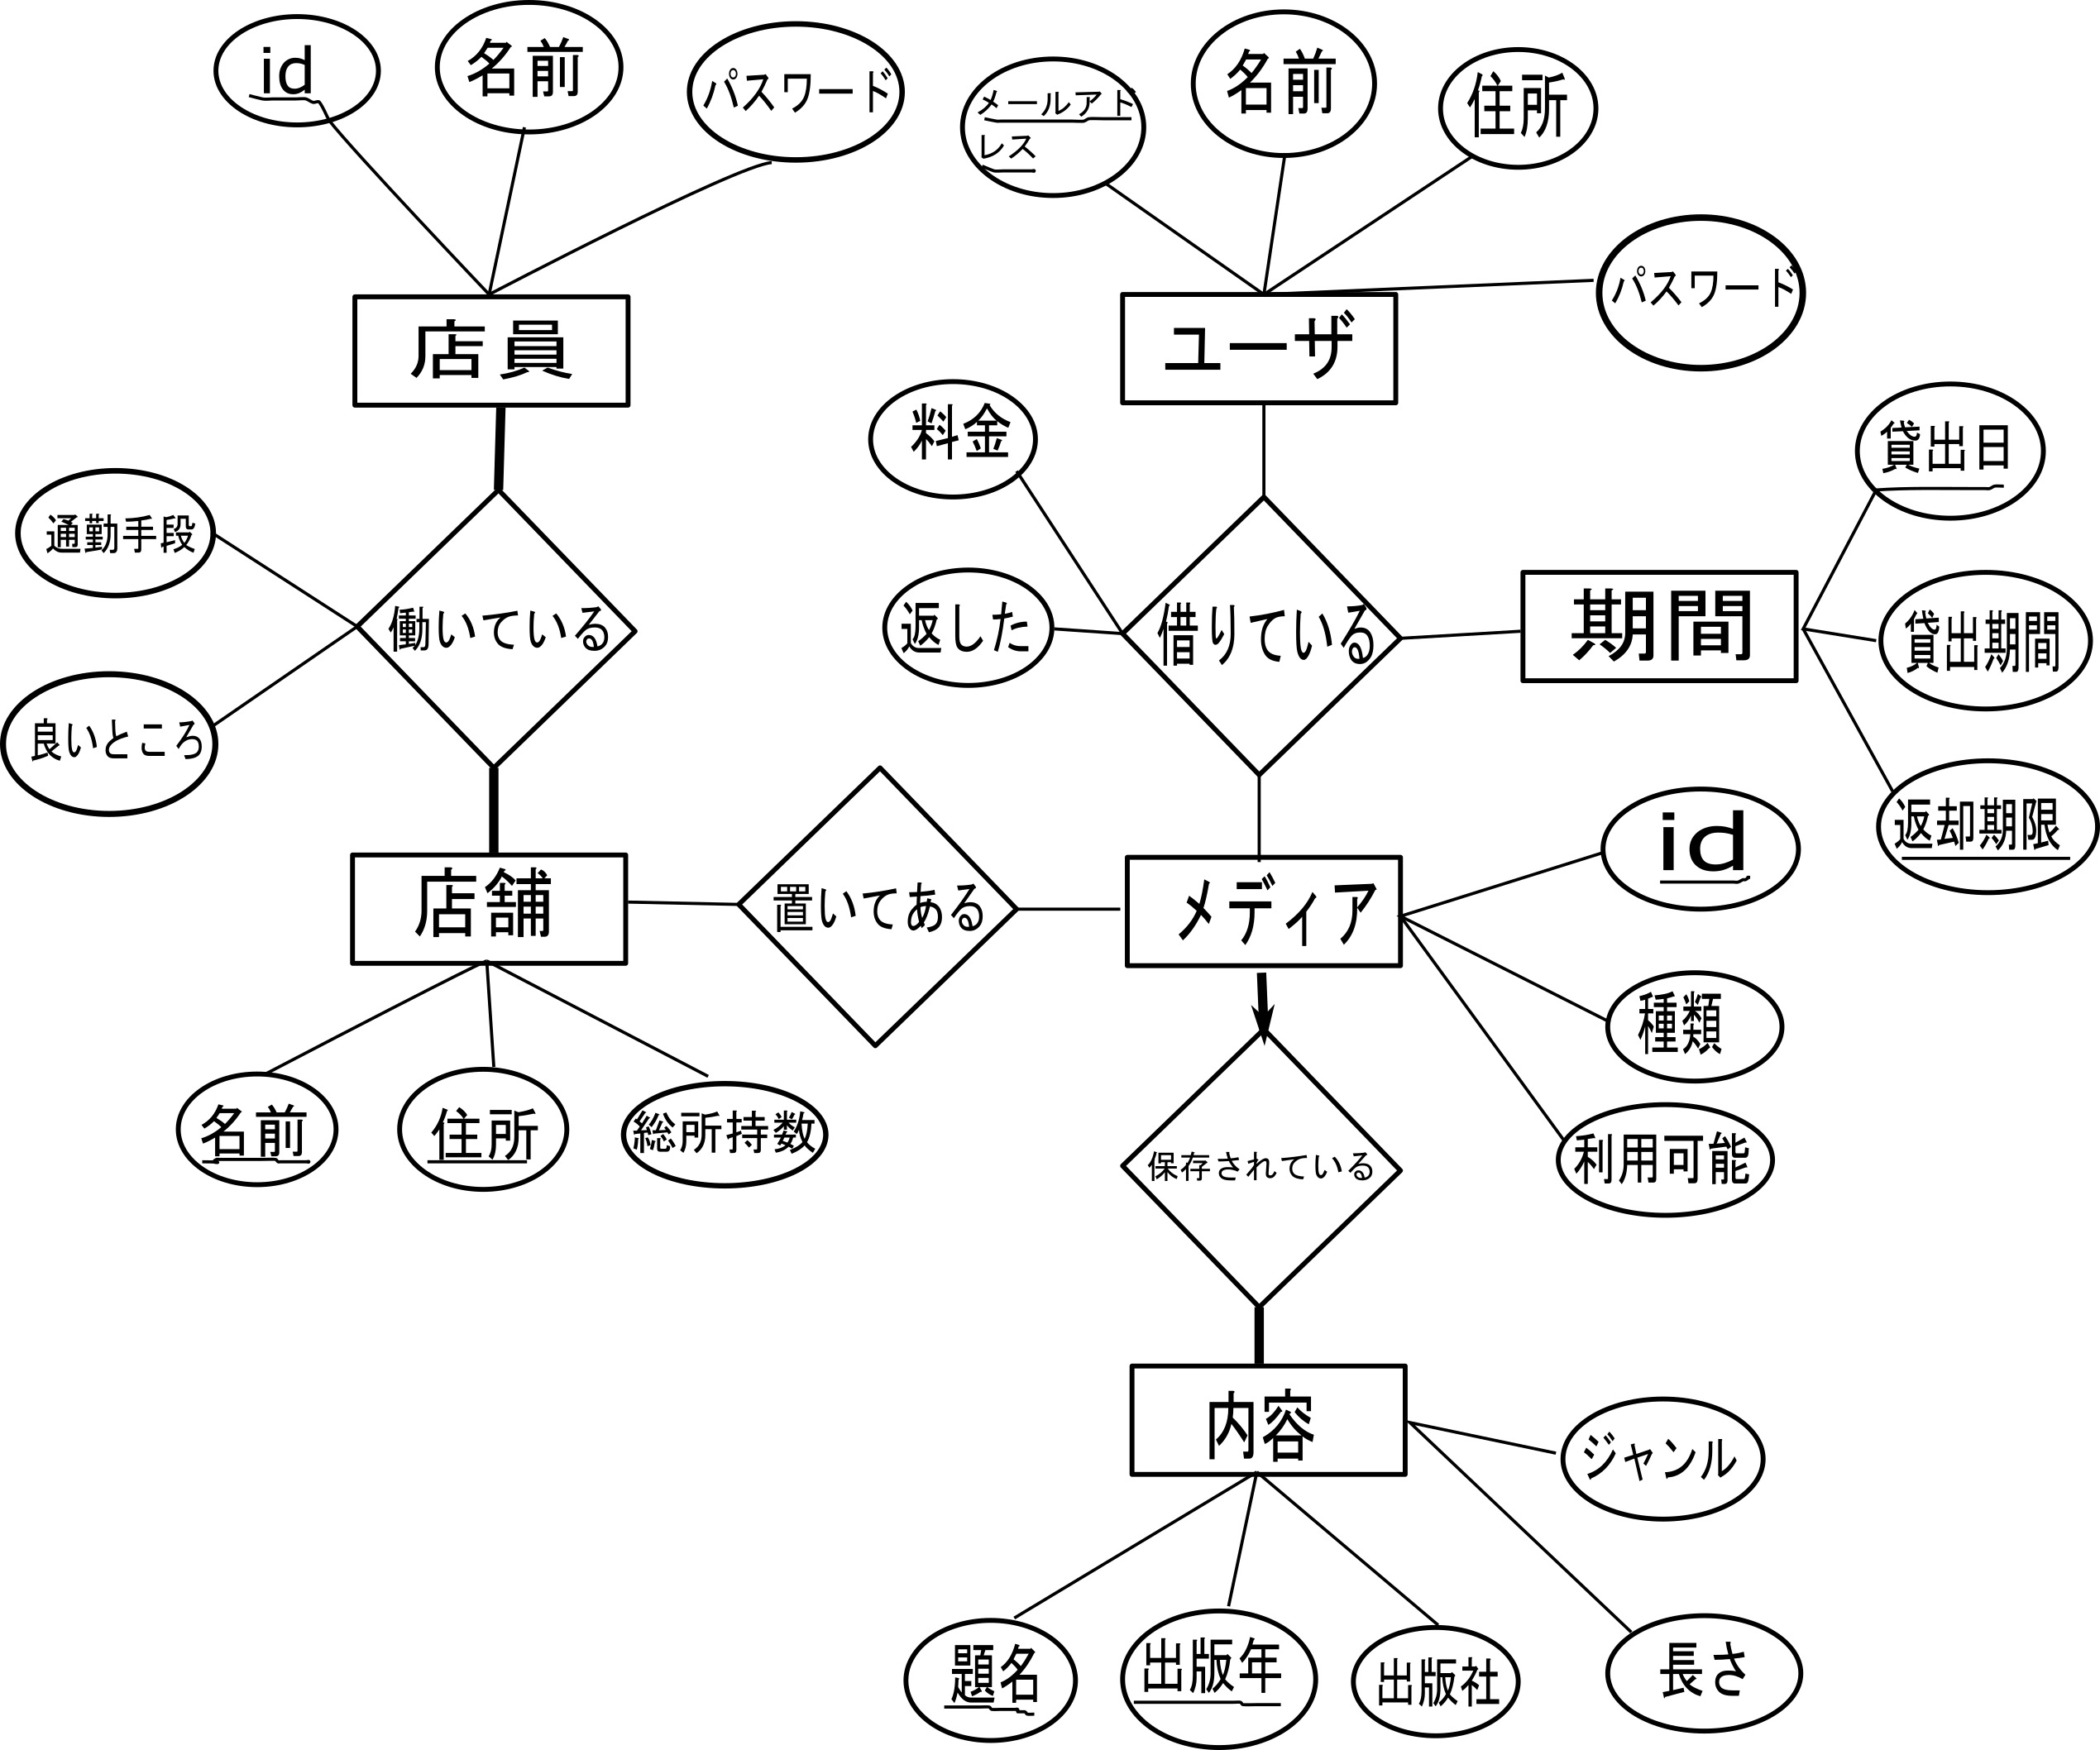
\includegraphics[scale=0.2]{ER_final.png}
\end{center}
\caption{実体関連図}
\label{fig:er}
\end{figure}
実体関連図は図1のようになった. 基本的には課題1のものと同じである. しかし, 異なる点もいくつかある.
\begin{description}
\item[パスワードの追加] \leavevmode \\
ユーザと店員の属性に「パスワード」を追加した. これはインタフェースを分けるためにログインする必要があるためである.
\item[関連「借りている」の三項関連化] \leavevmode \\
課題1のものだと同じユーザが同じメディアを二回借りることができなかったので, 
日付や期間に関する情報を属性ではなく実体として三項関連にした.
\item[属性「返した」と「利用可能」の追加] \leavevmode \\
ひとつのメディアが同時に借りられることのないように追加した.
\item[属性「最大数」と「数」の削除] \leavevmode \\
これは「メディア」ではなく「内容」に関する情報であるため, 「置いてある」の属性として不適切であったため削除した.
\item[属性「通勤手段」と「良いところ」の追加] \leavevmode \\
自明でない多値従属性を作るための属性である.
\end{description}

\section{関係スキーマ}
関係スキーマは以下のようになった.
\begin{itemize}
\item ユーザ(\underline{メールアドレス}, ユーザ名, ユーザ住所, ユーザパスワード)
\item メディア(\underline{mid}, 種類, 利用可能)
\item 内容(\underline{題名}, \underline{発売年}, 長さ, 出版社, ジャンル)
\item 店舗(\underline{店舗名}, \underline{店舗住所}, 総所持数)
\item 店員(\underline{eid}, 店員名, 店員パスワード)
\item 付属情報(\underline{通勤手段}, \underline{店の良い所})
\item 借りている(\underline{メールアドレス}, \underline{mid}, 料金, \underline{貸出日}, \underline{返却日}, 返した)
\item 期間(\underline{貸出日}, 貸出期間, \underline{返却日})
\item 置いてある(\underline{mid}, \underline{店舗名}, \underline{店舗住所})
\item 働いている1(\underline{eid}, \underline{店舗名}, \underline{店舗住所}, \underline{通勤手段})
\item 働いている2(\underline{eid}, \underline{店舗名}, \underline{店舗住所}, \underline{店の良い所})
\item 保存されている(\underline{mid}, \underline{題名}, \underline{発売年})
\end{itemize}
課題3のものに第2章で述べた変更点を反映させただけである. 全ての自明でない関数従属性の左辺は超キーであるからBoyce-Codd正規系である. それぞれのデータ例を以下に示す.
\begin{description}
\item[ユーザ(\underline{メールアドレス}, ユーザ名, ユーザ住所, ユーザパスワード)] \leavevmode \\
\begin{verbatim}
mail                 username useraddress userpw
-------------------- -------- ----------- ---------
yamada@example.jp    山田     A市         yamada
takahashi@example.jp 高橋     B市         takahashi
yoshida@example.jp   吉田     C市         yoshida
baba@example.jp      馬場     D市         baba
hotta@example.jp     堀田     E市         hotta
\end{verbatim}
\item[メディア(\underline{mid}, 種類, 利用可能)] \leavevmode \\
\begin{verbatim}
mid type    available
--- ------- ---------
1   VHS     yes
2   DVD     yes
3   DVD     yes
4   Blu-ray yes
5   Blu-ray yes
\end{verbatim}
\item[内容(\underline{題名}, \underline{発売年}, 長さ, 出版社, ジャンル)] \leavevmode \\
\begin{verbatim}
title published_year length         publisher genre
----- -------------- -------------- --------- -------
ABC   2000           01時間30分00秒 A         movie
ABD   2010           00時間50分30秒 B         drama
ACD   2005           02時間00分00秒 C         variety
BCD   2001           02時間00分00秒 D         anime
BE    2008           02時間10分00秒 E         sport
\end{verbatim}
\item[店舗(\underline{店舗名}, \underline{店舗住所}, 総所持数)] \leavevmode \\
\begin{verbatim}
shopname shopaddress total_media
-------- ----------- -----------
AAA      A市         1
ABD      B市         2
CAD      C市         2
EDC      D市         2
BCD      E市         3
\end{verbatim}
\item[店員(\underline{eid}, 店員名, 店員パスワード)] \leavevmode \\
\begin{verbatim}
eid clerkname clerkpw
--- --------- ---------
1   山田      yamada
2   高橋      takahashi
3   吉田      yoshida
4   馬場      baba
5   堀田      hotta
\end{verbatim}
\item[付属情報(\underline{通勤手段}, \underline{店の良い所})] \leavevmode \\
\begin{verbatim}
commute_method good_point_of_shop
-------------- ------------------
walk           A
walk           B
bicycle        A
bicycle        B
bus            A
\end{verbatim}
\item[借りている(\underline{メールアドレス}, \underline{mid}, 料金, \underline{貸出日}, \underline{返却日}, 返した)] \leavevmode \\
\begin{verbatim}
mail                 mid rental_fee rental_date return_date finished
-------------------- --- ---------- ----------- ----------- --------
yamada@example.jp    1   300        2019/01/04  2019/01/05  yes
takahashi@example.jp 2   300        2019/01/05  2019/01/06  yes
yoshida@example.jp   3   400        2019/01/06  2019/01/08  yes
baba@example.jp      4   400        2019/01/07  2019/01/09  yes
hotta@example.jp     5   500        2019/01/08  2019/01/11  yes
\end{verbatim}
\item[期間(\underline{貸出日}, 貸出期間, \underline{返却日})] \leavevmode \\
\begin{verbatim}
rental_date rental_duration return_date
----------- --------------- -----------
2019/01/04  1日             2019/01/05
2019/01/05  1日             2019/01/06
2019/01/06  2日             2019/01/08
2019/01/07  2日             2019/01/09
2019/01/08  3日             2019/01/11
\end{verbatim}
\item[置いてある(\underline{mid}, \underline{店舗名}, \underline{店舗住所})] \leavevmode \\
\begin{verbatim}
mid shopname shopaddress
--- -------- -----------
1   AAA      A市
2   ABD      B市
3   CAD      C市
4   EDC      D市
5   BCD      E市
\end{verbatim}
\item[働いている1(\underline{eid}, \underline{店舗名}, \underline{店舗住所}, \underline{通勤手段})] \leavevmode \\
\begin{verbatim}
eid shopname shopaddress commute_method
--- -------- ----------- --------------
1   AAA      A市         walk
2   ABD      B市         walk
3   CAD      C市         bicycle
4   EDC      D市         bicycle
5   BCD      E市         bus
\end{verbatim}
\item[働いている2(\underline{eid}, \underline{店舗名}, \underline{店舗住所}, \underline{店の良い所})] \leavevmode \\
\begin{verbatim}
eid shopname shopaddress good_point_of_shop
--- -------- ----------- ------------------
1   AAA      A市         A
2   ABD      B市         B
3   CAD      C市         A
4   EDC      D市         B
5   BCD      E市         A
\end{verbatim}
\item[保存されている(\underline{mid}, \underline{題名}, \underline{発売年})] \leavevmode \\
\begin{verbatim}
mid title published_year
--- ----- --------------
1   ABC   2000
2   ABD   2010
3   ACD   2005
4   BCD   2001
5   BE    2008
\end{verbatim}
\end{description}

\section{機能・インタフェース}
\subsection{ログイン}
\subsection{ユーザによる店舗検索}
\subsection{ユーザによる作品検索}
\subsection{ユーザによる履歴閲覧}
\subsection{店員によるユーザ登録}
\subsection{店員による貸出/返却}
\subsection{管理者による店員登録}
\subsection{管理者によるメディア登録}
\subsection{管理者による店舗登録/削除}
\subsection{管理者による店員の管理}
\subsection{管理者によるメディアの管理}

\section{工夫点}


\section{感想}



\end{document}
